\section{Flame sensor module}
\begin{figure}[H]
    \centering
    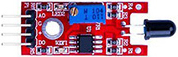
\includegraphics[angle=0, keepaspectratio=true, scale=1, width=200px, height=200px]{images/flame_sensor.jpg}
    %\caption{Caption}
\end{figure}
\subsection*{Description}
The flame sensor module detects infrared light (heat). This module has both analog and digital outputs. The strength of the signal received will depend on the intensity and distance of the flame.
\subsection*{Pin mapping}
This pin mapping corresponds to the pins from left to right with the module pins facing towards you.
\begin{table}[H]
    \centering
    \begin{tabular}{|c|c|c|c|c|}
    \hline
    Index &Label &Type &Name &Description\\ \hline
    0 &A0 &Analog output &A0 &Signal to activate relay \\ \hline
    1 &G &Ground &GND &\\ \hline
    2 &+ &Source voltage &$V+$ &Module source voltage ($5V$)\\ \hline
    3 &D0 &Digital output &D0 &\\ \hline
    \end{tabular}
    %\caption{Caption}
    %\label{tab:my_label}
\end{table}
\subsection*{Operation}
The output voltage pin at the analog pin (A0) is high and decreases towards zero when a flame is detected. A potentiometer on the module allows the adjustment of the sensor threshold. When the sensor reads a value above the threshold the digital pin (D0) is set to high.
\subsection*{Code}
Refer to listing \ref{python_flamesensor}.
%\lstinputlisting[caption=test]{laser.py}